\documentclass{acm_proc_article-sp}

\begin{document}

\title{Web Content Extraction Through Machine Learning
\titlenote{Source code for this project is avaiable on GitHub under the MIT License at https://github.com/ziyan/spider}}

\numberofauthors{2}
\author{
\alignauthor
Ziyan Zhou\\
\email{ziyanjoe@stanford.edu}
\alignauthor
Lei Sun\\
\email{sunlei@stanford.edu}
}

\maketitle

\begin{abstract}
Web content extraction is a key technology for enabling an array of applications aimed at understanding the web. While fully automated web extraction has been studied extensively, they often focuses on extracting structured data that appears in multiples on a single web page. This project aims to extract not-so-structured web content, like news articles, that appear only once in a noisy web pages. Our approach tries to cluster text blocks by their visual features from multiple similar pages from the same site, identify the useful clusters through simple NLP analysis, and generate content extraction rules that efficiently applies to future pages from the same site. Experiment shows that this method can achieve similar near-perfect accuracy as do other state-of-art approaches.

\end{abstract}

\keywords{Unsupervised learning, web scraping}

\section{Introduction}

Understanding the web is hard. The idea of semantic web, dating back almost to the invention of the web, that the various parts of web pages should be tagged such that machines as well as humans can make inferences based on the information they contain, has never gotten very far. Nowadays, the problem has worsen due to the increased complexity in web technology that came with better human interfaces and more creative designs. Even though various new semantic web technologies have been hyped up again in recent years, for example RSS and Open Graph, there remains the central problem of requiring content to be formatted twice, once for the machines benefit and once for the actual humans.

On the other hand, it is trivial for a parser to extract the underlying content of a web page when it is told the structure of the page. But as the number of website increases exponentially, it is hard, even impossible to analyze all websites manually one by one, not to mention that the page structure for a known site could be changing over time. 

Fortunately, web pages on the same site often share very similar structures. These pages are usually generated and presented by a content management system with some web templates and a structured data source backend. Humans are intrinsically good at discerning the common structure of these web pages, and with some experience, can quickly locate the relevant content on a complex page.

Given a set of similar pages from a specific site, the goal of this project is to teach machines to discover the underlying structure of the pages through unsupervised learning based on visual features, and then to extract the vital information while filtering out distractions.

\section{Previous Works}

Fully automated web content extraction has been studied extensively. A survey by Laender at el.\cite{laender:brief} systematically covers a wide range of techniques used for this purpose. These tools range from wrapper development to NLP-based and modeling-based approach. Some of the modeling-based approach and wrapper induction approach requires supervised learning methods like labeling sample dataset. Miao at el.\cite{gengxin:extracting} proposed a fully automatic tag path clustering approach to extract structures on a single page.

We wanted a simpler approach to this problem that does not require labeled training data while also maintaining site and domain agnostic. We also wanted to extract not-so-structured data like web articles that usually have variable length and appear standalone on web pages. Therefore, clustering multiple similar pages on the same site seems a reasonable good approach.

\section{Data Collection}

The training and testing dataset are extracted from popular English news article sites on the Internet, including site like theverge.com, npr.org, usatoday.com.\footnote{While originally being in the proposal, nytimes.com is later dropped from the dataset due to its subscription restriction leading to a lack of training examples.}

We devised two separate data collection methods for this project.

\subsection{Standalone Method}

The first one is a local machine based approach. 15 to 25 most recently published article pages are chosen from each of the sites. Each of these pages are then downloaded and rendered in a virtual webkit browser.\footnote{The collected data using the standalone method is available at https://github.com/ziyan/spider/tree/master/data}

By rendering the full page in a virtual browser, javascript can be injected to efficiently inspect elements on the page. Text enclosing blocks are first identified. For each text element, the algorithm finds its closest parent element that are displayed as block, such that inline links and other text decorators are not individually identified. Instead, their common parent element, which might be a paragraph is identified as a whole. For each chosen block, a set of features are then extracted, including the size and position of the block, the contained text, the font configurations, color, line height, tag path, etc. In fact, there are some 300 different CSS properties for each block. Our algorithm automatically extracts those with a non-default value. Therefore, the number of features varies from block to block in the data collection phase.

\subsection{Bookmarklet Method}

To enable a wider range of site collections and to enlist the help of crowds, we developed a bookmarklet that can be easily installed on user browsers.\footnote{The bookmarklet demonstration site is available at http://ziyan.github.io/spider/} The bookmarklet works by injecting javascript to the current active webpage. Essentially the same javascript code used in the standalone approach can now run inside user's browser. The extracted data is automatically uploaded to our server for clustering. This approach allowed us to collect some 400 pages from 60 different sites in a 48 hour period and offload some heavy workload and bandwidth need to user browsers.\footnote{The collected data using the bookmarklet method is available at https://spider.ziyan.net/store/}

\section{Clustering Blocks}

Each CSS property collected for the text blocks can be treated as discrete variables. These variables are vectorized by creating new feature dimension for each unique value and assigning 0 or 1 depending on whether the particular value is present in the property. Using this method, the features for each text block within the same site are normalized to the same length.

We noticed that text blocks on the page are not necessarily clustered together shaping like a gaussian distribution. Rather similar text blocks, like navigational buttons horizontally distributed across the top of the page, can cluster together in any shape. We also noticed some noisy elements only appears once on some of the pages. Furthermore, it is unclear how many cluster there will be since it depends heavily on the specific layout design of the web page. Therefore, we have chosen DBSCAN\cite{ester:dbscan}, density-based spatial clustering of applications with noise, as our clustering algorithm, which handles the the problem of unknown number of clusters, unknown shape of clusters and noise quite nicely..\footnote{The cluster outputs using DBSCAN are also available at https://github.com/ziyan/spider/tree/master/data}

Using this approach, we found that DBSCAN can quite accurately cluster the text blocks on the training dataset. To our surprise, the clustering results showed the body text of the articles across multiple pages, which is usually consist of paragraphs, are clustered all together in a single cluster. The navigational links are also clustered together, as well as the links in the footers. Other common elements on the pages, like similar sidebar, advertisement, comments, etc., are similarly also successfully clustered. Given all the visual features represented by the CSS properties, the algorithm is quite effective in discerning the different visual elements on the pages.

\section{Scoring Clusters}
Although all the blocks have been clustered quite precisely based on their visual properties, it is not trivial to find out which cluster the body text blocks reside in for a couple of reasons.

First, unlike the K-mean algorithm which requires the number of clusters to be specified in the beginning, the DBSCAN algorithm views clusters as areas of high density separated by areas of low density. So it is hard to predict how many clusters we will have in the output, and even if we know this information in advance, the order the output clusters are not guaranteed, thus there is no way to know which clusters are the ones that contain the body text we need, especially our data is the webpages from completely different domains with high complexity and high variance. For our training set, the number of output clusters ranges from a couple of clusters to more than 20.

What makes this task even harder is, it is very likely that the body text are classified into several different clusters, and the number of the ``useful'' clusters is unknown to us. The reason is that some sections of the body text have different CSS styles from others. For some domain in our training data set, for example, we notice there is one cluster containing all the quotes, and another containing all the bullet lists from different pages. For some domain, there is only one useful cluster containing what we need. But the number increases for visually stunning news website designed with quotations and fancy section titles.

Fortunately, most website has some metadata in order to accommodate Google's web crawler or Facebook's Open Graph. So we can extract the title and the description of an article by parsing the metadata of this page. These metadata usually contains a brief summary or just the first few words of the article content. With them, we are able to calculate the similarity between each cluster and these description and titles.

First we need to do some preprocessing to our raw text string before calculating similarity.

\makeatletter
\renewcommand{\theenumi}{\roman{enumi}}
\makeatother
\begin{enumerate}
\item Lowercase: convert all characters to lowercase
\item Tokenize: convert the sentences into a list of english words by splitting it with spaces and other punctuation marks.
\item Remove stop words: stop words are most common words in English, such as "of", "the" and "is". They appear in almost every document, thus provides little information to us.
\item Stemming: stemming is the process for reducing inflected or sometimes derived words to their stem, base or root form. e.g., the words "doing", "did" and "does" to the root word, "do". An open source stemmer is used in our project.
\end{enumerate}

With all the pre-processing done, we calculate the similarity with the tf-idf technique widely used in information retrieval area\cite{christopher:introduction}, which is defined as:
\begin{displaymath}
tfidf(t,d,D) = tf(t, d) \times idf(t, D)
\end{displaymath}
where $tf(t, d)$ is the term frequency, i.e.the number of times that term t occurs in document d, and
\begin{displaymath}
idf(t, D) = log\frac{|D|}{|\{d \in D : t \in d\}|}
\end{displaymath}

with \newline
- $|D|$: the total number of documents in the corpus \newline
- $|\{d \in D : t \in d\}|$: number of documents where the term t appears 

This algorithm performs very well in our system. For our training data, most of the non-body text such as ``Share This Article On Twitter'' has zero score because they appear in each web page. Some other text, like the title of a related article, have some similar words but get really low score compared the real body text. They both can be differentiated from the body text.

Below is an example score for a given page, whose description is: \textit{In a preliminary study, a new type of vaccine offers strong protection against malaria when given at high doses. The study was extremely small and short-term. But health leaders say they are cautiously optimistic about the approach.}

Some of the text along with their similarity score with the description are listed in the Table 1. Note that only text 4 and 5 are what should be extracted from this page. In our learning system, all the text in the same cluster will get a similarity score with descriptions, and the blocks whose score are higher than a threshold will be outputted as the body text we want to extract from the page.

\begin{table}
\caption{Frequency of Special Characters}
\begin{tabular}{  p{0.8cm}  p{6.7cm}  }
Score & Text Block \\
\hline
0.0 & Share article on Facebook, Twitter, Google+, Email, Comment \\
\hline
0.0 & Please keep your community civil. All comments must follow the  NPR.org Community rules  and  terms of use, and will be moderated prior to posting. NPR reserves the right to use the comments we receive, in whole or in part, and to use the commenter's name and location, in any medium. See also the  Terms of Use  Privacy Policy  and  Community FAQ \\
\hline
6.60 & More From Shots - Health News \\
\hline
49.98 & Previous experimental vaccines have shown some effectiveness against the malaria parasite, but none have provided high levels of protection against the disease. In November, another candidate vaccine showed  disappointing results  in tests among young infants, though it provided children moderate protection against the parasite. \\
\hline
64.27 & The experimental vaccine offered strong protection against malaria when given at high doses, scientists report Thursday in the journal Science. \\
\end{tabular}
\end{table}

\section{Generating Extraction Rules}

As the number of training examples increases, the clustering algorithm can take upwards of minutes to complete while the ranking of clusters converges as little additional information is accumulated with the addition of more similar pages. Clearly, content extraction cannot scale well when each page takes minutes to process. Therefore, for sites that are already fully learned, we devise a way to generate ``rules'' that enables content extraction without running the whole feature extraction, clustering and scoring pipeline.

During the data extraction phase, the CSS selector path is collected for each text block extracted. These selectors contains type, ID and any CSS classes for each element on the tree path to the text block, and can be used to almost uniquely locate the text block given the same web page. For example, a CSS selector may look like this:

\begin{verbatim}
body > div#a-386.article > div.p1 > p.p1.paragraph
\end{verbatim}

Once the clusters are scored, we consolidate the CSS selectors for all text blocks within the chosen clusters using a simple algorithm: given two selectors, if the number of elements on the path is the same, we go through each element and take an intersect of the sets of IDs and the sets of classes, therefore combining the two into one selector by eliminating the differences. This process is repeated for every pair of selectors in the clusters.

\begin{verbatim}
body > div#a-386.article > div.p1 > p.p1.paragraph
body > div#a-2383.article > div.p9 > p.p9.paragraph
\end{verbatim}

For example, the above two selectors can be consolidated into one:

\begin{verbatim}
body > div.article > div > p.paragraph
\end{verbatim}

With the consolidated rules, future content extraction can be made instant by simply applying the CSS selectors. In fact, our bookmarklet highlights content on the page in user browser using these consolidated CSS selectors while it also always extract and upload text blocks for the benefit of online training that is done in a task queue on the server. Although the user might not immediately benefits from the added new page, this approach eliminates the waiting time and provides a better bookmarklet experience.

Information can be lost while using this method to consolidate css selectors. But in practice, modern web pages usually have complicated structure and rarely produces such conflict. And we believe it is a fair tradeoff between accuracy and efficiency.

\section{Result Evaluation}

\begin{figure*}
\centering
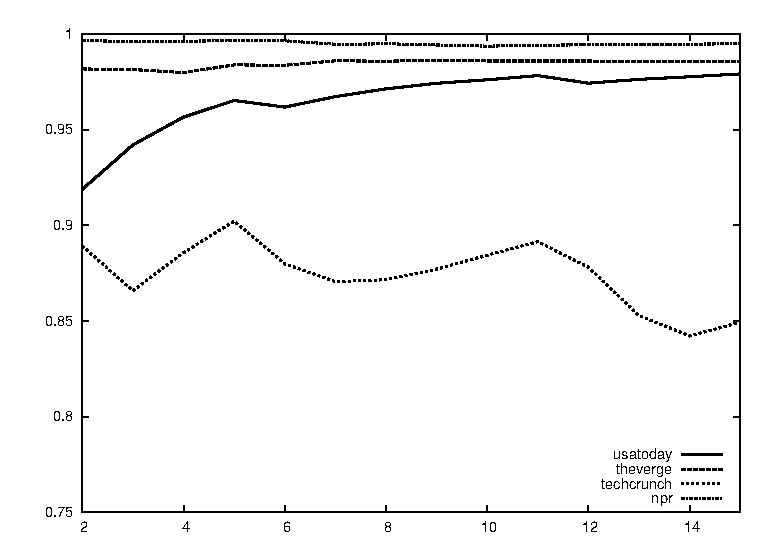
\epsfig{file=accuracy.eps}
\caption{Accuracy of our approach given different training sample set compared to data from DiffBot}
\end{figure*}

To evaluate the accuracy of our approach, we use third-party data from DiffBot\cite{diffbot}, a commercially available article crawling platform, as a non-bias reference. We compare text from the most likely cluster with the highest score to the text extracted by DiffBot for every page. The matching ratio is computed by finding the edit distance between the pair of word sequences. And then a percentage accuracy is calculated by averaging the matching ratios for all pages.

Using a new set of URLs for each site, the accuracy is calculated for different training sample sizes ranging from 2 pages to 15 pages. See \emph{Figure 1}. We found that generally the accuracy improves as we increase the size of training dataset.\footnote{Data from DiffBot as well as accuracy evaluator used for graphing are also available on the project's GitHub repository.}

As shown in \emph{Figure 1}, in the cases of npr.org, theverge.com and usatoday.com, the accuracy of our approach averages 99.5\%, 98.4\% and 96.6\% respectively.

In the case of techcrunch.com, our accuracy drops to 87.4\%. This is because techcrunch happens to use a different visual style for its blockquotes in the articles. And our accuracy evaluation only considers the top scored cluster while the blockquotes and the paragraphs for techcrunch have landed in different clusters due to their visual differences. Note we also don't have a particular order when adding new page to the training set, therefore, pages with more ``abnormal'' content can be added at any point, causing the fluctuation in the accuracy.

Improvements in selecting all the correct clusters will greatly help us improve our accuracy and they are discussed in the \emph{Future Directions} section.

\section{Future Directions}

\subsection{Selecting Clusters using a Bounding Box}

Once the clusters are scored using our method, we can be fairly certain that the majority of the content resides in the top scored cluster. The difficulty lies in selecting other clusters that might have partial contents. These clusters may include section headers, blockquotes, lists, tables, etc. that are not visually similar to the main content.

One approach to this problem would be to create a bounding box for the top scored cluster since we extracted all positional and dimensional information regarding each text blocks. We can then use this bounding box to label other clusters with non-zero scores that might fall within it. Since we throw away zero-scored clusters, inline advertisements are unlikely to be included by this bounding box, however, links to related articles that are really related can be mistakenly included as part of the content.

\subsection{Language Agnostic}

The current NLP approach only works for English articles. This is because text segmentation is exponentially harder for other languages like Chinese. However, we might be able to use a ngram approach to apply the term frequency inverse document frequency algorithm.

\subsection{Reinforced Learning}

Currently, our bookmarklet interface does not allow the user to provide feedback on what is highlighted correctly or incorrectly. If the user interface incorporate some sort of feedback, we can use the feedback to conduct reinforced learning to improve our feature selection and cluster selection.

\section{Conclusion}
Our results show that clustering text blocks across multiple pages based on visual features does work quite effectively. This approach has proven to be simple, efficient and scalable. It is also likely that improvement can be made to achieve perfect web article extraction.

\bibliographystyle{abbrv}
\bibliography{report}

\end{document}

